\subsection{Lines in Space}


The idea of a `straight line' is something anyone can understand intuitively.
For instance, any person can say that the edge of a rectangular tabletop forms 
a `straight line', and we would all agree. Similarly, ask any person to draw a `straight line', and they would know what to do.
In this section, rather than relying on intuition, we shall introduce a \textit{mathematical model} for what we call
a `straight line'. This is done in the context of the Model for Space that was introduced in Unit 1.2.

\vspace{1em}

The concept of a ‘straight line’ is closely related to that of ‘betweenness’. Intuitively, if
 three points in space lie on a ‘straight line’, then one of the three points lies somewhere ‘between’ the
 other two. In order to motivate our definition of a straight line, we therefore first consider
 what it means for a point $\bar{r}$ to be ‘between’ two points $\bar{p}$ and $\bar{q}$.


\begin{definitionbox}
\textbf{Betweenness of Points in Space}

Let $\bar{p}, \bar{q}, \bar{r} \in \mathbb{R}^3$. We say that $\bar{r}$ is \textit{between} $\bar{p}$ and $\bar{q}$ if and only if
for some $0 < t < 1$, 
\[
  \bar{r} = (1 - t) \bar{p} + t \bar{q}.
\]

\end{definitionbox}

From our experiences with reality, we understand that the distance between two points on a `straight line' is the shortest, 
unless an intermediate point lies exactly along that line. Expressing this in terms of our model we have that, given three points $\bar{p}, \bar{q}, \bar{r}$ in space:\\
 $\|\bar{p} - \bar{q}\| < \|\bar{p} - \bar{r}\| + \|\bar{r} - \bar{q}\|$ if $\bar{r}$ is not between $\bar{p}$ and $\bar{q}$, and
$\|\bar{p} - \bar{q}\| = \|\bar{p} - \bar{r}\| + \|\bar{r} - \bar{q}\|$ \\ if $\bar{r}$ is between $\bar{p}$ and $\bar{q}$.
As a motivation for our definition of betweenness, we show that this fact is true in our model for space.

\begin{theorembox}
  Let $\bar{p}, \bar{q}, \bar{r} \in \mathbb{R}^3$ such that $\bar{p} \neq \bar{q}, \bar{p} \neq \bar{r}, \bar{r} \neq \bar{q}$.

  Then $||\bar{p} - \bar{q}|| = ||\bar{p} - \bar{r}|| + ||\bar{r} - \bar{q}||$ if and only if $\exists t \in (0,1)$ such that $\bar{r} = (1 - t) \bar{p} + t \bar{q}$.

\end{theorembox}

\begin{proofbox}
  
We shall first show that if $\|\bar{q}-\bar{p}\| = \|\bar{q}-\bar{r}\| + \|\bar{r}-\bar{p}\|$, then
$\exists t \in \mathbb{R}$, $0 < t < 1$ such that $\bar{r} = t\bar{p} + (1-t)\bar{q}$. 

Assume $\|\bar{q}-\bar{p}\| = \|\bar{q}-\bar{r}\| + \|\bar{r}-\bar{p}\|$.\\
Then $||\bar{q}-\bar{p}\|^2 = (\|\bar{q}-\bar{r}\| + \|\bar{r}-\bar{p}\|)^2 $

$= \|\bar{q}-\bar{r}\|^2 + 2\|\bar{q}-\bar{r}\|\|\bar{r}-\bar{p}\| + \|\bar{r}-\bar{p}\|^2$ \hfill (A)

\vspace{1em}

By definition of the norm, the commutativity and distributivity of the dot product, we have

\quad $\|\bar{q} - \bar{p}\|^2 = \|(\bar{q} - \bar{r}) + (\bar{r} - \bar{p})\|^2$

\quad $= [(\bar{q} - \bar{r}) + (\bar{r} - \bar{p})] \cdot [(\bar{q} - \bar{r}) + (\bar{r} - \bar{p})]$

\quad $= [(\bar{q} - \bar{r}) + (\bar{r} - \bar{p})] \cdot (\bar{q} - \bar{r}) + [(\bar{q} - \bar{r}) + (\bar{r} - \bar{p})] \cdot (\bar{r} - \bar{p})$

\quad $= (\bar{q} - \bar{r}) \cdot (\bar{q} - \bar{r}) + (\bar{r} - \bar{p}) \cdot (\bar{q} - \bar{r}) + (\bar{q} - \bar{r}) \cdot (\bar{r} - \bar{p}) + (\bar{r} - \bar{p}) \cdot (\bar{r} - \bar{p})$

\quad $= |\bar{q} - \bar{r}\|^2 + 2(\bar{q} - \bar{r}) \cdot (\bar{r} - \bar{p}) + \|\bar{r} - \bar{p}\|^2$ \hfill (B)

Combining (A) and (B) we have\\
$\|\bar{q}-\bar{r}\|\|\bar{r}-\bar{p}\| = (\bar{q}-\bar{r}) \cdot (\bar{r}-\bar{p})$. \hfill (C)

\hfill $\qed$
\end{proofbox}

\begin{proofbox}

By the Cauchy-Schwarz inequality, it follows that\\
$\exists a \in \mathbb{R}$ such that $\bar{q}-\bar{r} = a(\bar{r}-\bar{p})$ \hfill (D)

i.e. $a = \frac{\bar{q}-\bar{r}}{\bar{r}-\bar{p}}$

\vspace{1em}

Since $\bar{r} \neq \bar{p}, \bar{r} \neq \bar{q}$, it follows that \\
$\|\bar{r}-\bar{p}\| > 0$ and $\|\bar{q}-\bar{r}\| > 0$.\\
$\therefore a = \frac{\|\bar{q}-\bar{r}\|}{\|\bar{r}-\bar{p}\|} > 0$

\vspace{1em}

Isolating $\bar{r}$ in (D) we find that\\
$\bar{r} = \left(\frac{a}{1+a}\right)\bar{p} + \left(1-\frac{a}{1+a}\right)\bar{q}$

\vspace{1em}

Since $a > 0$, it follows that $0 < \frac{a}{1+a} < 1$.

Now let $t = \frac{a}{1+a}$, then $t \in \mathbb{R},$ and $0 < t < 1$.\\
Hence $\bar{r} = tp + (1-t)\bar{q}$.

\vspace{1em}

Now we shall prove the inverse; that is, if $\bar{r} = t\bar{p} + (1 - t)\bar{q}$ for some $t \in \mathbb{R},\ 0 < t < 1$,  
then $\|\bar{q} - \bar{p}\| = \|\bar{q} - \bar{r}\| + \|\bar{r} - \bar{p}\|$.

\vspace{1em}

Suppose that $\exists\, t \in \mathbb{R}$ such that $\bar{r} = t\bar{p} + (1 - t)\bar{q}$.

\vspace{1em}

Then:

$\|\bar{q} - \bar{r}\| = \|\bar{q} - t\bar{p} - (1 - t)\bar{q}\|$\\
\quad $= \|\bar{q} - t\bar{p} - \bar{q} + t\bar{q}\|$ \hfill [Distributivity over scalar addition] \\
\quad $= \|-t(\bar{p} - \bar{q})\|$ \hfill [Distributivity over Vector Subtraction] \\
\quad $= t \cdot \|\bar{p} - \bar{q}\| = t \cdot \|\bar{q} - \bar{p}\|$ \hfill [Positive Definiteness of the Norm]

\vspace{1em}

And:

$\|\bar{r} - \bar{p}\| = \|t\bar{p} + (1 - t)\bar{q} - \bar{p}\|$\\
\quad $= \|t\bar{p} - \bar{p} + (1 - t)\bar{q}\|$ \hfill [Associativity of vector addition] \\
\quad $= \|-(1 - t)(\bar{p} - \bar{q})\|$ \hfill [Distributivity of scalar multiplication] \\
\quad $= (1 - t) \cdot \|\bar{p} - \bar{q}\| = (1 - t) \cdot \|\bar{q} - \bar{p}\|$ \hfill [Positive  Definiteness of the Norm]

\vspace{1em}

Now we have:

$\|\bar{q} - \bar{r}\| + \|\bar{r} - \bar{p}\|$

\quad $= t\|\bar{q} - \bar{p}\| + (1 - t)\|\bar{q} - \bar{p}\|$

\quad $= \|\bar{q} - \bar{p}\|$

\hfill \qed

\end{proofbox}

\newpage

We shall now illustrate the notion of betweenness at the hand of an example.

\begin{examplebox}

  \setstretch{1.5} 

  Let $\bar{p}, \bar{q}, \bar{r} \in \mathbb{R}^3$ such that 
  $\bar{p} = \langle -4, -1, 1 \rangle, \bar{q} = \langle 2,1,3 \rangle, \bar{r} = \langle-1,0,2 \rangle$.\\
  Determine whether the points $\bar{r}$ and $\bar{0}$ are between $\bar{p}$ and $\bar{q}$.

  \vspace{1em}

  \textbf{Solution:}

  \vspace{1em}

  By definition of betweenness, $\bar{0}$ is between $\bar{p}$ and $\bar{q}$ if and only if for some constant $0 < t < 1$,

  $\bar{0} = t\bar{p} + (1 - t)\bar{q}$.

  \quad $= \langle 2-6t, 1-2t, 3-2t \rangle$

  \vspace{0.5em}

  Hence, by definition of vector equality, $\bar{0}$ is between $\bar{p}$ and $\bar{q}$ if and only if for some constant $0 < t < 1$,
  $0 = 2-6t, 0 = 1-2t, 0= 3-2t$.

  \quad $0 = 2-6t \Rightarrow t = \frac{1}{3}$, but

  \quad $0 = 1-2t \Rightarrow t = \frac{1}{2}$.

  Since $\frac{1}{3} \neq \frac{1}{2}$, there is no value for $t$ that satisfies the condition.

  Therefore, $\bar{0}$ is not between $\bar{p}$ and $\bar{q}$.

  Now $\bar{r}$ is between $\bar{p}$ and $\bar{q}$ if and only if for some constant $0 < t < 1$,

  $\bar{r} = t\bar{p} + (1 - t)\bar{q}$.

  \quad $= \langle 2-6t, 1-2t, 3-2t \rangle$

  \vspace{0.5em}

  Hence, by definition of vector equality, $\bar{r}$ is between $\bar{p}$ and $\bar{q}$ if and only if for some constant $0 < t < 1$, 
  $-1 = 2-6t, 0 = 1-2t, 2 = 3-2t$.

  \quad $-1 = 2-6t \Rightarrow \frac{1}{2}$
 
  \quad $0 = 1-2t \Rightarrow t = \frac{1}{2}$.

 \quad  $2 = 3-2t \Rightarrow t = \frac{1}{2}$.

  Hence $\bar{r} = \frac{1}{2}\bar{p} + (1 - \frac{1}{2})\bar{q}$.

  Since $0 < \frac{1}{2} < 1$, it follows that $\bar{r}$ is between $\bar{p}$ and $\bar{q}$.

\end{examplebox}


Now we can define a `straight line' in our model of space. As mentioned previously, if 
three points are colinear; that is, they lie on a `straight lie', we expect that one of them
must be an intermediate point between the other two.

\begin{definitionbox}
\textbf{A Straight Line in Space}

  A line is a set $L$ of points in the form

  \[
    L = \{t\bar{p} + (1 - t)\bar{q} : t \in \mathbb{R} \}
  \]

  where $\bar{p}, \bar{q} \in \mathbb{R}^3$ and $\bar{p} \neq \bar{q}$.

\end{definitionbox}

\begin{notebox}

  Consider a line $L = \{t\bar{p} + (1 - t)\bar{q} : t \in \mathbb{R}\}$ in $\mathbb{R}^3$.

  \begin{enumerate}
    \item $L$ is a set in $\mathbb{R}^3$. A point $\bar{x}$ is \textbf{either} an element of $L$, or it is \textbf{not} an element of $L$.\\
          So say that $\bar{x} \in L.$ Then we say that `$\bar{x}$ \textbf{is a point on $L$'}, or that `$\bar{x}$ \textbf{lies on $L$'}.

    \item Both $\bar{p}$ and $\bar{q}$ are elements of $L$. We therefore refer to $L$ as `\textbf{the line through} $\bar{p}$ \textbf{and} $\bar{q}$'.
    
    \item By the definition of betweenness of points in space, a point $\bar{x} \in \mathbb{R}^3$ is on $L$ if and only if
          $\bar{x} = (1 - t)\bar{p} + t\bar{q}$ for some $t \in \mathbb{R}$. Therefore, we speak of a line determined by the equation \\
          $\bar{x} = (1 - t)\bar{p} + t\bar{q}$ for some $t \in \mathbb{R}$.
          Equivalently, the equation can be written as \\
          $\bar{x} = \bar{q} + t(\bar{p} - \bar{q})$ for some $t \in \mathbb{R}$.

    \item $L$ has more than one equation, in the form describe in point 3. Furthermore, a single
     line can be described using infinitely many different equations.

  \end{enumerate}
\end{notebox}

Our intuition of what a `straight line' is, is further proven to be in agreement with our model for space in the following theorem:

\begin{theorembox}

  Let $L$ be a line in $\mathbb{R}^3$. If $\bar{p}, \bar{q}, \bar{r} \in \mathbb{R}^3$, then exactly one of the following statements is true:

  \begin{enumerate}[label=(\arabic*)]

    \item $\bar{p}$ is between $\bar{r}$ and $\bar{q}$.

    \item $\bar{q}$ is between $\bar{r}$ and $\bar{p}$.

    \item $\bar{r}$ is between $\bar{p}$ and $\bar{q}$.

  \end{enumerate}

\end{theorembox}
  
\begin{proofbox}

  Let  $\bar{p}, \bar{q}, \bar{r} \in \mathbb{R}^3$ be points on $L$.

  We shall first show that at most one of (1), (2), or (3) is true.

  Assume, for contradiction, that (1) and (2) are both true. Then, by definition of betweenness,\\
  $\exists s,t \in \mathbb{R}$ where $s,t \in (0,1)$ that satisfy

  $\bar{p} = t\bar{p} + (1 - t)\bar{r}$ and $\bar{q} = s\bar{p} + (1 - s)\bar{r}$.

  \vspace{1em}

  Since $0 < t < 1$, $\bar{p} = t\bar{q} + (1 - t)\bar{r}$

  $\Rightarrow \bar{r} = \frac{\bar{p}-s\bar{q}}{1-t}$ \hfill (A)

  Similarly, since $0 < s < 1$, $\bar{q} = s\bar{p} + (1 - s)\bar{r}$

  $\Rightarrow \bar{r} = \frac{\bar{p}-t\bar{q}}{1-s}$ \hfill (B)

  \vspace{1em}

  Equating (A) and (B) we have

  $\frac{\bar{p}-s\bar{q}}{1-t} = \frac{\bar{p}-t\bar{q}}{1-s}$

  \quad $\Rightarrow (1-s)(\bar{p}-t\bar{q}) = (1-t)(\bar{q}-s\bar{p})$ \hfill [Multiplying by $(1-s)$ and $(1-t)$ on both sides]

  \quad $\Rightarrow (\bar{p}-t\bar{q}) - s(\bar{p}-t\bar{q}) = (\bar{q}-s\bar{p})-t(\bar{q}-s\bar{p})$ \hfill [Distributivity over Scalar Subtraction]

  \quad $\Rightarrow \bar{p} - t\bar{q} - s\bar{p} + st\bar{q} = \bar{q} - s\bar{p} - t(\bar{p} + st\bar{p}$ \hfill [Distributivity over Scalar Subtraction]

  \quad $\Rightarrow \bar{p} - st\bar{p} = \bar{q} - st\bar{q}$ 

  \quad $(1-st)\bar{p} = (1-st)\bar{q}$ \hfill [Distributivity over Scalar Subtraction]

  \vspace{1em}

  Note that by assumption, 
  
  $0 < t < 1 \Rightarrow 0 < st < s$ \hfill [Multiplying by s on all sides]

  \quad $\Rightarrow -s < -st < 0$ \hfill [Multiplying by -1 on all sides]

  \quad $\Rightarrow 1-s < 1-st < 1$ \hfill [Adding 1 to all sides].

  Now $1-s>0$

  $\therefore 1-s < 1-st$

  \quad $\Rightarrow 1-st > 1-s > 0$

  \quad $\Rightarrow 1-st > 0$

  \quad $\Rightarrow \bar{p} = \bar{r}$, contradicting our assumption that $\bar{p} \neq \bar{r}$ \hfill [Def. of Betweenness]

  Therefore (1) and (2) cannot both be true. In the same way, (1) and (3) cannot both be true, and, (2) and (3) cannot both be true. 
  Therefore at most one of (1), (2) and (3) is true.

  \vspace{1em}

  Now we show that at least one of (1), (2) and (3) is true.

  Assume that $\bar{x} = \bar{u} + t\bar{v}, t \in \mathbb{R}$ is an equation for $L$. Since $\bar{p}, \bar{q}, \bar{r} \in \mathbb{R}, \exists t_0, t_1, t_2 \in \mathbb{R}$ that satisfy $\bar{p}=\bar{u} +t_0\bar{v}$, $\bar{q}=\bar{u} +t_1\bar{v}$, and $\bar{r}=\bar{u} +t_2\bar{v}$.

  Since $\bar{p} \neq \bar{q}$, $\bar{q} \neq \bar{r}$ and $\bar{p} \neq \bar{r}$, it follows that $t_0 \neq t_1$, $t_1 \neq t_2$ and $t_0 \neq t_1$.

  Now there are three possibilities to consider:

  \begin{enumerate}
    \renewcommand{\labelenumi}{(\roman{enumi})}
    \item $t_0 < t_1 < t_2$ or $t_2 < t_1 < t_0$
    \item $t_0 < t_2 < t_1$ or $t_1 < t_2 < t_0$
    \item $t_1 < t_0 < t_2$ or $t_2 < t_0 < t_1$
  \end{enumerate}
  \hfill $\qed$
\end{proofbox}

\begin{proofbox}

  Consider case (i), and suppose that $t_0 < t_1 < t_2$.

  Then $t_0\bar{v} < t_1\bar{v} < t_2\bar{v}$ \hfill [Scalar Multiplication preserves order since $\bar{v}$ is fixed]

  \quad $\Rightarrow \bar{u} + t_0\bar{v} < \bar{u} + t_1\bar{v} < \bar{u} + t_2\bar{v}$ \hfill [Adding $\bar{u}$ to all sides]

  \quad $\Rightarrow \bar{p} < \bar{q} < \bar{r}$ \hfill [By definition of $\bar{p}, \bar{q}, \bar{r}$]

  Hence, $\bar{q}$ lies between $\bar{p}$ and $\bar{r}$.

  A similar argument applies to cases (ii) and (iii). We thus obtain the following implications:
  \begin{enumerate}
    \renewcommand{\labelenumi}{(\roman{enumi})}
    \item If $t_0 < t_1 < t_2$ or $t_2 < t_1 < t_0$, then $\bar{q}$ is between $\bar{p}$ and $\bar{r}$.
    \item If $t_0 < t_2 < t_1$ or $t_1 < t_2 < t_0$, then $\bar{r}$ is between $\bar{p}$ and $\bar{q}$.
    \item If $t_1 < t_0 < t_2$ or $t_2 < t_0 < t_1$, then $\bar{p}$ is between $\bar{q}$ and $\bar{r}$.
  \end{enumerate}

  This shows that at least one of (i), (ii), or (iii) must be true. However, it has already been established that at most one of them can be true.

  Therefore, exactly one of (i), (ii), or (iii) is true.

  \hfill $\qed$

\end{proofbox}

Given a line $L$ in $\mathbb{R}^3$, there are two important kinds of subsets of $L$: \textit{line segments} and \textit{rays}.

\begin{definitionbox}
  \textbf{Line Segment}

  Consider distinct points $\bar{p}$ and $\bar{q}$ in $\mathbb{R}^3$. The \textit{line segment} between
  $\bar{p}$ and $\bar{q}$ is the set of points

  \[
    S = \{t\bar{p} + (1 - t)\bar{q} : 0 \leq t \leq 1 \}.
  \]
\end{definitionbox}

\begin{remarkbox}
  The line segment $S$ between two points $\bar{p}$ and $\bar{q}$ in $\mathbb{R}^3$ consists of the points $\bar{p}$ and $\bar{q}$ \textbf{and} all points $\bar{x}$ 
  between $\bar{p}$ and $\bar{q}$. In particular, a point $\bar{x}$ is between $\bar{p}$ and $\bar{q}$ if and only if
  $\bar{x} \in S$ and $\bar{x} \neq \bar{p}$ and $\bar{x} \neq \bar{q}$.
\end{remarkbox}

\begin{definitionbox}
  \textbf{Ray}

  Consider distinct points $\bar{p}$ and $\bar{q}$ in $\mathbb{R}^3$. A \textit{ray} is a set of points of the form
  \[
    R = \{t\bar{p} + (1 - t)\bar{q} : t \geq 0\} =\{\bar{q} + t(\bar{p} - \bar{q}) : t \geq 0\}.
  \]

  The point $\bar{q}$ is called the \textit{origin} of the ray.
\end{definitionbox}

\begin{remarkbox}
  Let $L$ be a line in space.

  \begin{enumerate}
    \item Any point $\bar{q} \in L$ divides $L$ exactly into two rays.

    Let $\bar{p}$ and $\bar{r}$ be two points on $L$ such that $\bar{q}$ is between $\bar{p}$ and $\bar{r}$.
    
    Then $R_1 = \{\bar{q} + t(\bar{p} - \bar{q}) : t \geq 0\}$ and $R_2 = \{\bar{q} + t(\bar{r} - \bar{q}) : t \geq 0\}$ are 
    two rays with origin $\bar{q}$ such that:

    \[
      L = R_1 \cup R_2  \quad \text{and} \quad R_1 \cap R_2 = \{\bar{q}\}.
    \]

    %Image1.tex
% This file is part of the WTW124 course material.


\begin{center}
\begin{tikzpicture}[scale=0.8]
    % Define the coordinates of the endpoints
    \coordinate (R1_end) at (1, -1);
    \coordinate (R2_end) at (-2, 2);

    % Draw the arrowed line from R2 to R1
    \draw[{Stealth[length=3mm, width=2mm]}-{Stealth[length=3mm, width=2mm]}, thick] (R2_end) -- (R1_end);


    % Calculate and place points along the line using interpolation
    \path let \p1 = (R2_end), \p2 = (R1_end) in
        coordinate (r_point) at ($(\p1)!0.15!(\p2)$)
        coordinate (q_point) at ($(\p1)!0.45!(\p2)$)
        coordinate (p_point) at ($(\p1)!0.8!(\p2)$);

    % Draw the points
    \fill (r_point) circle (3pt) node[left=5pt] {$\bar{r}$};
    \fill (q_point) circle (3pt) node[left=5pt] {$\bar{q}$};
    \fill (p_point) circle (3pt) node[left=5pt] {$\bar{p}$};

    % Label the endpoints
    \node[below right] at (R1_end) {$R_1$};
    \node[above left] at (R2_end) {$R_2$};
\end{tikzpicture}
\end{center}

  \item If $\bar{x} \in L$, then $\bar{x} \in R_1$ if and only if $\bar{x}$ is on the line segment between $\bar{p}$ and $\bar{q}$, or
        $\bar{p}$ is between $\bar{q}$ and $\bar{x}$. We therefore refer to $R_1$ as the ray with origin $\bar{q}$ in the direction of
        $\bar{p}$, and call $(\bar{p} - \bar{q})$ the direction vector of $R_1$.

        \begin{center}
\begin{tikzpicture}[scale=1.2]

  % Define endpoints
  \coordinate (R1) at (2.5, -2.5);
  \coordinate (Q)  at (0, 0);

  % Draw the line with arrow from q to R1
  \draw[-{Stealth[length=3mm, width=2mm]}, thick] (Q) -- (R1);

  % Point p in between q and R1
  \path let \p1 = (Q), \p2 = (R1) in
    coordinate (P) at ($(\p1)!0.6!(\p2)$);

  % Mark points
  \fill (Q) circle (2pt) node[left=5pt] {$\bar{q}$};
  \fill (P) circle (2pt) node[left=5pt] {$\bar{p}$};
  \node[below right] at (R1) {$R_1$};

  % Coordinates for where to place equation labels
  \path let \p1 = (Q), \p2 = (P) in
    coordinate (Eq1) at ($(\p1)!0.35!(\p2)$);

  \path let \p1 = (P), \p2 = (R1) in
    coordinate (Eq2) at ($(\p1)!0.5!(\p2)$);

  % Draw closed dots at the equation positions
  \fill (Eq1) circle (2pt);
  \fill (Eq2) circle (2pt);

  % Add equations
  \node[right=10pt] at (Eq1) 
    {$\bar{x} = \bar{q} + t(\bar{p} - \bar{q}),\ 0 < t < 1$};

  \node[right=10pt] at (Eq2) 
    {$\bar{x} = \bar{q} + t(\bar{p} - \bar{q}),\ t > 1$};

\end{tikzpicture}
\end{center}

        
  \item For any two points $\bar{p}$ and $\bar{q}$ in $\mathbb{R}^3$, the set $R = \{\bar{q}+t\bar{p} : t \geq 0\}$ is a ray. Indeed,
  
  \[R=\{\bar{q}+t([\bar{p}+\bar{q}] - \bar{q}) : t \geq 0\}.\]
  Therefore $R$ is the ray with origin $\bar{q}$ in the direction of $\bar{p}+\bar{q}$.
  
  \end{enumerate}
\end{remarkbox}

\newpage
The following table shows how the concepts of lines, rays, line segments and betweenness
 are related to one another.
\begin{notebox}
  \[
\bar{x} = t\bar{p} + (1 - t)\bar{q}
\]

\begin{tabular}{|>{\centering\arraybackslash}m{3.5cm}
                |>{\centering\arraybackslash}m{3.5cm}
                |>{\centering\arraybackslash}m{3.5cm}
                |>{\centering\arraybackslash}m{3.5cm}|}
\hline
\textbf{Line ($t \in \mathbb{R}$)} &
\textbf{Ray ($t \geq 0$)} &
\textbf{Line segment ($0 \leq t \leq 1$)} &
\textbf{Between ($0 < t < 1$)} \\
\hline


% 1. Line
\vspace{1em}
\begin{tikzpicture}
\draw[{Stealth[length=3mm, width=2mm]}-{Stealth[length=3mm, width=2mm]}] (-1.2,0) -- (1.2,0);
\fill (-0.7,0) circle (2pt) node[below] {$\bar{q}$};
\fill (0.7,0) circle (2pt) node[below] {$\bar{p}$};
\end{tikzpicture} &

% 2. Ray
\vspace{1em}
\begin{tikzpicture}
\draw[-{Stealth[length=3mm, width=2mm]}] (-0.7,0) --(1.2,0);
\fill (-0.7,0) circle (2pt) node[below] {$\bar{q}$};
\fill (0.7,0) circle (2pt) node[below] {$\bar{p}$};
\end{tikzpicture} &

% 3. Line segment
\vspace{1em}
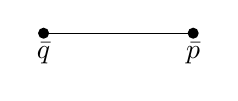
\begin{tikzpicture}
\draw[-] (-0.7,0) -- (1.2,0);
\fill (-0.7,0) circle (2pt) node[below] {$\bar{q}$};
\fill (1.2,0) circle (2pt) node[below] {$\bar{p}$};
\end{tikzpicture} &

% 4. Between
    \vspace{1em}
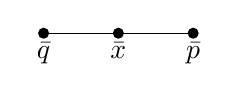
\begin{tikzpicture}
\draw[-] (-0.7,0) -- (1.2,0);
\fill (-0.7,0) circle (2pt) node[below] {$\bar{q}$};
\fill (0.25,0) circle (2pt) node[below] {$\bar{x}$};
\fill (1.2,0) circle (2pt) node[below] {$\bar{p}$};
\end{tikzpicture} \\

\hline
\end{tabular}

\end{notebox}

\begin{examplebox}

Determine whether the points 
$\bar{a} = \langle 5, -3, 6 \rangle$ and 
$\bar{b} = \langle -4, -1, -3 \rangle$ are on the line $L$ through
$\bar{p} = \langle 2, -1, 3 \rangle$ and
$\bar{q} = \langle -1, 1, 0 \rangle$.

\vspace{1em}

\textbf{Solution} 

\vspace{1em}
A point $\bar{x} \in \mathbb{R}^3$ lies on $L$ if and only if
\[
\bar{x} = \bar{q} + t(\bar{p} - \bar{q}) = \langle 3t - 1,\ 1 - 2t,\ 3t \rangle \quad \text{for some } t \in \mathbb{R}.
\]

Therefore, by the definition of vector equality, $\bar{a} = \langle 5, -3, 6 \rangle$ lies on $L$ if and only if there exists $t \in \mathbb{R}$ such that:
\[
\begin{aligned}
5 &= 3t - 1 \\
-3 &= 1 - 2t \\
6 &= 3t
\end{aligned}
\]

From the third equation, $3t = 6$ implies $t = 2$. Substituting into the first two:
\[
3(2) - 1 = 6 - 1 = 5 \quad \text{and} \quad 1 - 2(2) = 1 - 4 = -3
\]

So all three equations are satisfied with $t = 2$. Therefore, $\bar{a} \in L$.

Now consider $\bar{b} = \langle -4, -1, -3 \rangle$. This point lies on $L$ if there exists $t \in \mathbb{R}$ such that:
\[
\begin{aligned}
-4 &= 3t - 1 \\
-1 &= 1 - 2t \\
-3 &= 3t
\end{aligned}
\]

From the third equation, $3t = -3$ implies $t = -1$. Substituting into the second equation:
\[
1 - 2(-1) = 1 + 2 = 3 \ne -1
\]

So $t = -1$ satisfies the third equation but not the second. Hence, no single $t$ satisfies all three equations. Therefore, $\bar{b} \notin L$.

\end{examplebox}
\begin{examplebox}
Determine whether or not the points \(\bar{b} = \langle 0, 3, 0 \rangle\) and \(\bar{c} = \left\langle \frac{3}{2}, 0, \frac{3}{2} \right\rangle\) are on the line segment \(S\) between the points \(\bar{p} = \langle 1, 1, 1 \rangle\) and \(\bar{q} = \langle 2, -1, 2 \rangle\).
\vspace{1em}

\textbf{Solution} 
\vspace{1em}

For a point \(\bar{x}\), we have
\[
\bar{x} \in S \iff \bar{x} = t\bar{p} + (1 - t)\bar{q} \quad \text{for some } 0 \leq t \leq 1.
\]

Hence, the point \(\bar{b} = \langle 0, 3, 0 \rangle\) is on the line segment \(S\) if and only if there exists a real number \(0 \leq t \leq 1\) such that
\[
\bar{b} = t\bar{p} + (1 - t)\bar{q} = \langle 2 - t, 2t - 1, 2 - t \rangle.
\]

So \(\bar{b} \in S\) if and only if the following equations are satisfied:
\[
0 = 2 - t, \quad 3 = 2t - 1, \quad 0 = 2 - t.
\]

From the first equation, we get \(t = 2\). This value of \(t\) also satisfies the second and third equations, so:
\[
\bar{b} = 2\bar{p} + (1 - 2)\bar{q}.
\]

Therefore, \(\bar{b}\) is on the line through \(\bar{p}\) and \(\bar{q}\). However, \(t = 2 > 1\), so \(\bar{b}\) is not on the line segment \(S\) between \(\bar{p}\) and \(\bar{q}\).

Now consider the point \(\bar{c} = \left\langle \frac{3}{2}, 0, \frac{3}{2} \right\rangle\). This point is on \(S\) if and only if
\[
\bar{c} = t\bar{p} + (1 - t)\bar{q} = \langle 2 - t, 2t - 1, 2 - t \rangle \quad \text{for some } 0 \leq t \leq 1.
\]

Thus, \(\bar{c} \in S\) if and only if
\[
\frac{3}{2} = 2 - t, \quad 0 = 2t - 1, \quad \frac{3}{2} = 2 - t.
\]

The first equation implies \(t = \frac{1}{2}\). This value also satisfies the other equations. Therefore,
\[
\bar{c} = \frac{1}{2} \bar{p} + \left(1 - \frac{1}{2}\right) \bar{q}.
\]

Since \(0 \leq \frac{1}{2} \leq 1\), it follows that \(\bar{c} \in S\).
\end{examplebox}

In the following examples we investigate the intersection of lines in space
$L_1 = \left\{ \bar{q} + t(\bar{p} - \bar{q}) : t \in \mathbb{R} \right\}$ and $L_2 = \left\{ \bar{b} + s(\bar{a} - \bar{b}) : s \in \mathbb{R} \right\}$
in space intersect at a point \(\bar{x}\) if and only if \(\bar{x} \in L_1 \cap L_2\). That is, the lines intersect at \(\bar{x}\) if and only if both
$\bar{x} = \bar{q} + t(\bar{p} - \bar{q})$ for some $t \in \mathbb{R}$ and $\bar{x} = \bar{b} + s(\bar{a} - \bar{b})$ for some  $s \in \mathbb{R}.$

Note that it is possible for \(L_1\) and \(L_2\) to:
\begin{itemize}
  \item intersect at exactly one point,
  \item not intersect at all (e.g., parallel lines), or
  \item intersect at infinitely many points (if they coincide).
\end{itemize}
\begin{examplebox}
Consider the line \(L_1\) through \(\bar{p} = \langle 1, 0, 1 \rangle\) and \(\bar{q} = \langle 0, 2, 0 \rangle\), and the line \(L_2\) through the points \(\bar{a} = \langle 2, 1, 2 \rangle\) and \(\bar{b} = \langle 0, 3, 0 \rangle\). 

Determine whether or not \(L_1\) and \(L_2\) intersect, and find all points of intersection, if any exist.

\vspace{1em}

\textbf{Solution}

\vspace{1em}

The lines \(L_1\) and \(L_2\) intersect at a point \(\bar{x} = \langle x, y, z \rangle\) if and only if \(\bar{x} \in L_1\) and \(\bar{x} \in L_2\). Therefore, \(L_1\) and \(L_2\) intersect at \(\bar{x}\) if and only if
\[
\bar{q} + t(\bar{p} - \bar{q}) = \bar{x} = \bar{b} + s(\bar{a} - \bar{b}) \quad \text{for some } t, s \in \mathbb{R}. \tag{i}
\]

It then follows from the definition of vector equality that
\[
t = x = 2s, \qquad 2 - 2t = y = 3 - 2s, \qquad t = z = 2s.
\]

The third equation implies that \(t = 2s\). Substituting \(t = 2s\) into the second equation yields:
\[
2 - 2(2s) = 3 - 2s \quad \Rightarrow \quad -2s = 1 - 2s \quad \Rightarrow \quad s = -\frac{1}{2}.
\]

Hence \(t = 2s = -1\). These values for \(s\) and \(t\) also satisfy the first equation, since
\[
t = -1 = 2\left(-\frac{1}{2}\right) = 2s.
\]

Therefore, these are the only values for \(t\) and \(s\) that satisfy (i). Thus, \(L_1\) and \(L_2\) intersect at the single point
\[
\bar{x} = \bar{q} - (\bar{p} - \bar{q}) = \langle -1, 4, -1 \rangle.
\]
\end{examplebox}

\begin{examplebox}
Determine whether or not the lines \(L_1 = \{ \langle 1 - t, 1 - t, 2t \rangle : t \in \mathbb{R} \}\) and 

\(L_2 = \{ \langle s, 2, s - 1 \rangle : s \in \mathbb{R} \}\) intersect, and find the points of intersection, if any exist.

\vspace{0.5em}

\textbf{Solution}

\vspace{0.5em}

The lines \(L_1\) and \(L_2\) intersect at a point \(\bar{x} = \langle x, y, z \rangle\) if and only if \(\bar{x} \in L_1\) and \(\bar{x} \in L_2\). Therefore, \(L_1\) and \(L_2\) intersect at \(\bar{x}\) if and only if
\[
\langle 1 - t, 1 - t, 2t \rangle = \bar{x} = \langle s, 2, s - 1 \rangle \quad \text{for some } t, s \in \mathbb{R}. \tag{i}
\]

From the definition of vector equality, it follows that
\[
1 - t = x = s, \qquad 1 - t = y = 2, \qquad 2t = z = s - 1.
\]

The second equation implies that \(t = -1\). Substituting \(t = -1\) into the first equation gives:
\[
s = 1 - (-1) = 2.
\]

Substituting \(t = -1\) into the third equation yields:
\[
2(-1) = -2 = s - 1 \quad \Rightarrow \quad s = -1.
\]

Since \(2 \neq -1\), it follows that there are no real numbers \(t\) and \(s\) that satisfy (i). Therefore, the lines \(L_1\) and \(L_2\) do not intersect.
\end{examplebox}

\begin{examplebox}
  Let $L_1$ be the line with equation $\bar{x} = \langle 1 + t,\, 2 + t,\, 3 + t \rangle,\text{ } t \in \mathbb{R},$
and $L_2$ the line with equation $\bar{x} = \langle 2 - 2s,\, 3 - 2s,\, 4 - 2s \rangle, \text{ } s \in \mathbb{R}.$

Determine whether or not these lines intersect, and find the points of intersection, if any such points exist.

\vspace{0.5em}

\textbf{Solution}

\vspace{0.5em}

The lines $L_1$ and $L_2$ intersect at a point $\bar{x} = \langle x, y, z \rangle$ if and only if $\bar{x} \in L_1$ and $\bar{x} \in L_2$. Therefore, $L_1$ and $L_2$ intersect at $\bar{x}$ if and only if
\[
\langle 1 + t,\, 2 + t,\, 3 + t \rangle = \bar{x} = \langle 2 - 2s,\, 3 - 2s,\, 4 - 2s \rangle
\]
for some $t, s \in \mathbb{R}$.

It follows from the definition of vector equality that
\[
1 + t = x = 2 - 2s, \quad 2 + t = y = 3 - 2s, \quad 3 + t = z = 4 - 2s.
\tag{A}
\]

All three equations imply that $t = 1 - 2s.$ Hence for every real number $s$, there exists a real number $t = 1 - 2s$ such that $t$ and $s$ satisfy (A). 

Therefore, if 
$\bar{x} = \langle 2 - 2s,\, 3 - 2s,\, 4 - 2s \rangle \in L_2,$
then
$\bar{x} = \langle 1 + (1 - 2s),\, 2 + (1 - 2s),\, 3 + (1 - 2s) \rangle \in L_1.$

Conversely, if
$\bar{x} = \langle 1 + t,\, 2 + t,\, 3 + t \rangle \in L_1,$
then
$\bar{x} = \left\langle 2 - 2 \cdot \frac{1 - t}{2},\, 3 - 2 \cdot \frac{1 - t}{2},\, 4 - 2 \cdot \frac{1 - t}{2} \right\rangle \in L_2.$


Therefore, $L_1 = L_2$ so that every point on the line is a point of intersection.

\end{examplebox}

Our observations of the physical world tell us that, given two points $\bar{p} \neq \bar{q}$, there is exactly one straight line through $\bar{p}$ and $\bar{q}$. Another way of expressing this fact is that if two lines $L_1$ and $L_2$ intersect in more than one point, then $L_1 = L_2$. In the following theorem, we prove that this is indeed the case. This result serves as a further motivation for our definition of a line in space.

\begin{theorembox}
  
  \textbf{Equality of Lines with Multiple Intersection Points}

If two lines $L_1$ and $L_2$ intersect at more than one point, then $L_1 = L_2$.
\end{theorembox}

% LineEqualityProof.tex
% This file contains the proof

\begin{proofbox}
Let \( L_1 = \{ t\bar{p} + (1 - t)\bar{q} : t \in \mathbb{R} \} \)  
and \( L_2 = \{ s\bar{a} + (1 - s)\bar{b} : s \in \mathbb{R} \} \).  

Assume that \( L_1 \) and \( L_2 \) intersect at two distinct points, say \( \bar{u} \) and \( \bar{v} \),  
with \( \bar{u} \ne \bar{v} \). Let \( L \) be the line through \( \bar{u} \) and \( \bar{v} \).  

We shall show that \( L_1 = L = L_2 \).  

\vspace{1em}

Since \( \bar{u}, \bar{v} \in L_1 \), there exist \( t_0, t_1 \in \mathbb{R} \) such that  
\[
\bar{u} = t_0\bar{p} + (1 - t_0)\bar{q}, \quad
\bar{v} = t_1\bar{p} + (1 - t_1)\bar{q}.
\]
Since \( \bar{u} \ne \bar{v} \), it follows that \( t_0 \ne t_1 \).  

\vspace{1em}

Now consider a point
\[
\bar{x} = r(t_0\bar{p} + (1 - t_0)\bar{q}) + (1 - r)(t_1\bar{p} + (1 - t_1)\bar{q}).
\]
By the properties of vector addition and scalar multiplication,
\begin{align*}
\bar{x}
&= \big( rt_0 + (1 - r)t_1 \big) \bar{p}
+ \big( r(1 - t_0) + (1 - r)(1 - t_1) \big) \bar{q} \\
&= \big( rt_0 + t_1 - rt_1 \big) \bar{p}
+ \big( r - rt_0 + 1 - r - (1 - t_1) \big) \bar{q} \\
&= \big( rt_0 + t_1 - rt_1 \big) \bar{p}
+ \big( 1 - (rt_0 + t_1 - rt_1) \big) \bar{q}.
\end{align*}
Hence \( \bar{x} \in L_1 \). But \( \bar{x} \) was a point on the line through \( \bar{u} \) and \( \bar{v} \),  
so this shows every point on the line \( L \) lies in \( L_1 \).  

\vspace{1em}

Now, using the identities:
\[
\bar{u} = t_0\bar{p} + (1 - t_0)\bar{q}, \quad
\bar{v} = t_1\bar{p} + (1 - t_1)\bar{q},
\]
we multiply both by \( t_1 \) and \( t_0 \), respectively:
\begin{align*}
t_1\bar{u} &= t_1t_0\bar{p} + t_1(1 - t_0)\bar{q} \tag{A} \\
t_0\bar{v} &= t_0t_1\bar{p} + t_0(1 - t_1)\bar{q} \tag{B}
\end{align*}


\end{proofbox}
\begin{proofbox}
Subtracting (B) from (A):
\begin{align*}
t_1\bar{u} - t_0\bar{v}
&= t_1(1 - t_0)\bar{q} - t_0(1 - t_1)\bar{q} \\
&= \big( t_1 - t_0 \big)\bar{q} \\
\Rightarrow \quad \bar{q} &= \frac{t_1\bar{u} - t_0\bar{v}}{t_1 - t_0}
= \frac{t_0}{t_1 - t_0} \bar{u} - \frac{t_1}{t_1 - t_0} \bar{v} \tag{C}
\end{align*}

\vspace{1em}


Likewise, observe:
\begin{align*}
\bar{u} - \bar{v}
&= (t_0 - t_1)\bar{p} + (1 - t_0 - (1 - t_1))\bar{q} \\
&= (t_0 - t_1)\bar{p} + (t_1 - t_0)\bar{q} \\
&= (t_0 - t_1)(\bar{p} - \bar{q}) \\
\Rightarrow \quad \bar{p}
&= \frac{1 - t_0}{t_0 - t_1} \bar{u} - \frac{1 - t_1}{t_0 - t_1} \bar{v} \tag{D}
\end{align*}
    
Now suppose that \( \bar{y} \in L_1 \). Then \( \bar{y} = t\bar{p} + (1 - t)\bar{q} \) for some \( t \in \mathbb{R} \).  
Substitute from (C) and (D):
\begin{align*}
\bar{y}
&= t\left( \frac{1 - t_0}{t_0 - t_1} \bar{u} - \frac{1 - t_1}{t_0 - t_1} \bar{v} \right)
+ (1 - t) \left( \frac{t_0}{t_1 - t_0} \bar{u} - \frac{t_1}{t_1 - t_0} \bar{v} \right) \\
&= \left( \frac{t(1 - t_0)}{t_0 - t_1} + \frac{(1 - t)t_0}{t_0 - t_1} \right) \bar{u}
+ \left( -\frac{t(1 - t_1)}{t_0 - t_1} - \frac{(1 - t)t_1}{t_0 - t_1} \right) \bar{v} \\
&= \frac{t - t_1}{t_0 - t_1} \bar{u}
+ \left( 1 - \frac{t - t_1}{t_0 - t_1} \right) \bar{v}.
\end{align*}

Thus \( \bar{y} \in L \). So every point on \( L_1 \) lies on \( L \), i.e., \( L_1 \subseteq L \).  
By symmetry, the same argument shows \( L_2 \subseteq L \).  
Hence, \( L_1 = L = L_2 \).  
\hfill \( \qed \)
\end{proofbox}


\vspace{1em}
  As with parallel lines in coordinate geometry, we can also define parallel lines in our model for space:
  \begin{definitionbox}
    \textbf{Parallel Lines in Space}

    Two lines $L_1 = \{\bar{q} +t(\bar{p} - \bar{q}) : t \in \mathbb{R}\}$ and $L_2 = \{\bar{b} +t(\bar{a} - \bar{b}) : t \in \mathbb{R}\}$ are \textit{parallel} if and only if

    \[
      \bar{p}-\bar{q} = k(\bar{a}-\bar{b}) \text{ for some } k \in \mathbb{R} \text{ such that } k \neq 0.
    \]

  \end{definitionbox}

\begin{remarkbox}
 Consider the lines $L_1 = \{ \bar{q} + t(\bar{p} - \bar{q}) : t \in \mathbb{R} \}$ and $L_2 = \{ \bar{b} + t(\bar{a} - \bar{b}) : t \in \mathbb{R} \}$
in $ \mathbb{R}^3$.

If \( \alpha \) is a non-zero real number, then
\[
\bar{p} - \bar{q} = \alpha (\bar{a} - \bar{b}) \quad \text{if and only if} \quad
\bar{a} - \bar{b} = \frac{1}{\alpha}(\bar{p} - \bar{q}).
\]

Therefore, \( L_1 \) and \( L_2 \) are \textbf{parallel} if and only if
\[
\bar{a} - \bar{b} = \beta (\bar{p} - \bar{q}) \quad \text{for some non-zero real number } \beta.
\]

This essentially means that one vector is a scalar multiple of the other. Geometrically, the lines are parallel if they go in the same direction (or exactly opposite).
\end{remarkbox}
\vspace{1em}
Intuitively, if two distinct lines \( L_1 \) and \( L_2 \) are parallel, then \( L_1 \) and \( L_2 \) do not intersect.
In terms of our model of space, we can prove this idea, all while motivating our definition of parallel lines, with the following theorem:

\begin{theorembox}
  \textbf{Non-Intersection of Parallel Lines}

  If $L_1$ and $L_2$ are distinct parallel lines in $\mathbb{R}^3$, then they do not intersect.
\end{theorembox}

\begin{proofbox}
Let \( L_1 = \{ \bar{q} + t(\bar{p} - \bar{q}) : t \in \mathbb{R} \} \) and  
\( L_2 = \{ \bar{b} + s(\bar{a} - \bar{b}) : s \in \mathbb{R} \} \) be distinct parallel lines in \( \mathbb{R}^3 \). Since \( L_1 \neq L_2 \), and the lines are parallel, they do not coincide.  
Thus, we may assume (without loss of generality) that \( \bar{q} \notin L_2 \), i.e., $\bar{q} \neq \bar{b} + s(\bar{a} - \bar{b}) \text{ for all } s \in \mathbb{R}.$

\vspace{0.5em}

Since \( L_1 \) and \( L_2 \) are parallel, there exists a non-zero real number \( \alpha \) such that 

$\bar{p} - \bar{q} = \alpha(\bar{a} - \bar{b}).$
Therefore, it follows that $L_1 = \{ \bar{q} + \alpha t(\bar{a} - \bar{b}) : t \in \mathbb{R} \}$.

\vspace{0.5em}

Now suppose, for contradiction, that \( L_1 \) and \( L_2 \) intersect at some point \( \bar{x} \in \mathbb{R}^3 \).  
Then there exist \( t_0, s_0 \in \mathbb{R} \) that satisfy: 

$\bar{x} = \bar{q} + \alpha t_0 (\bar{a} - \bar{b}) = \bar{b} + s_0 (\bar{a} - \bar{b})$.

Subtracting \( \alpha t_0 (\bar{a} - \bar{b}) \) from both sides yields

\(\bar{q} = \bar{b} + s_0 (\bar{a} - \bar{b}) - \alpha t_0 (\bar{a} - \bar{b}) \\
\quad = \bar{b} + (s_0 - \alpha t_0)(\bar{a} - \bar{b}).
\)

\vspace{0.5em}
Now let \( s = s_0 - \alpha t_0 \). Then
\(
\bar{q} = \bar{b} + s(\bar{a} - \bar{b}),
\)
which implies \( \bar{q} \in L_2 \), evidently contradicting our earlier assumption that \( \bar{q} \notin L_2 \).
 
Hence, \( L_1 \) and \( L_2 \) do not intersect.

\hfill $\qed$
\end{proofbox}

\begin{notebox}
  The Theorem of Non-Intersection of Parallel Lines states that distinct parallel lines do not intersect.
  The converse of this theorem, however, is generally false. If two lines $L_1$ and $L_2$ do not intersect, it does not follow that they are parallel.
\end{notebox}
\begin{examplebox}
Let \( L_1 \) be the line through \( \bar{p} = \langle 2, 3, 1 \rangle \) and \( \bar{q} = \langle 4, 5, 5 \rangle \), and \( L_2 \) the line through \( \bar{a} = \langle -1, 1, 2 \rangle \) and \( \bar{b} = \langle 5, 7, 14 \rangle \). Determine whether or not \( L_1 \) and \( L_2 \) are parallel.

\vspace{0.5em}

\textbf{Solution}

\vspace{0.5em}

\( \bar{p} - \bar{q} = \langle -2, -2, -4 \rangle \) and \( \bar{a} - \bar{b} = \langle 6, 6, 12 \rangle \).  
Therefore  
\( \bar{a} - \bar{b} = \langle 6, 6, 12 \rangle = -3\langle -2, -2, -4 \rangle = -3(\bar{p} - \bar{q}) \).  
Therefore \( L_1 \) and \( L_2 \) are parallel.
\end{examplebox}

\begin{examplebox}
Let \( L_1 = \{\langle 1 - t, 1 - t, 2t \rangle : t \in \mathbb{R} \} \) and \( L_2 = \{\langle s, 2, s - 1 \rangle : s \in \mathbb{R} \} \).  
Given that \( L_1 \) and \( L_2 \) do not intersect, show that \( L_1 \) and \( L_2 \) are not parallel.

\vspace{0.5em}

\textbf{Solution}

\vspace{0.5em}

By the definition of vector addition, and scalar multiplication, \( L_1 \) and \( L_2 \) can be expressed as  
\[
L_1 = \{\langle 1, 1, 0 \rangle + t\langle -1, -1, 2 \rangle : t \in \mathbb{R} \}
\]
and  
\[
L_2 = \{\langle 0, 2, -1 \rangle + s\langle 1, 0, 1 \rangle : s \in \mathbb{R} \}.
\]

If \( L_1 \) and \( L_2 \) were parallel, then  
\(
\langle -1, -1, 2 \rangle = \alpha \langle 1, 0, 1 \rangle = \langle \alpha, 0, \alpha \rangle
\)
for some \( \alpha \in \mathbb{R} \).  
By the definition of vector equality, it is implied that \( -1 = 0 \), which is not true.  
Therefore \( L_1 \) and \( L_2 \) are not parallel.
\end{examplebox}

\begin{examplebox}
  Consider the points \(\bar{p} = \langle 1, 0, 2 \rangle\), \(\bar{q} = \langle c, 2, 1 \rangle\), \(\bar{a} = \langle 5, c, 3 \rangle\), and \(\bar{b} = \langle -7, -1, 1 \rangle\) in \(\mathbb{R}^3\), where \(c \in \mathbb{R}\) is a constant. We determine all values of \(c\), if any, so that the line through \(\bar{p}\) and \(\bar{q}\) is parallel to the line through \(\bar{a}\) and \(\bar{b}\).

\vspace{1em}

\textbf{Solution}

\vspace{1em}

By definition, the line through \(\bar{p}\) and \(\bar{q}\) is parallel to the line through \(\bar{a}\) and \(\bar{b}\) if and only if there exists a non-zero real number \(\alpha\) such that
\(
\bar{a} - \bar{b} = \alpha (\bar{p} - \bar{q}).
\)

We have
\(
\bar{a} - \bar{b} = \langle 12, c + 1, 2 \rangle \text{ and } \bar{p} - \bar{q} = \langle 1 - c, -2, 1 \rangle.
\)

Therefore, for a real number \(\alpha\), the equation \(\bar{a} - \bar{b} = \alpha (\bar{p} - \bar{q})\) holds if and only if
\[
12 = \alpha (1 - c), \quad c + 1 = -2\alpha, \quad \alpha = 2.
\]

According to the last equation, if \(\bar{a} - \bar{b} = \alpha (\bar{p} - \bar{q})\), then \(\alpha = 2\). Substituting \(\alpha = 2\) into the first and second equations yields
\[
12 = 2 (1 - c) \quad \text{and} \quad c + 1 = -4.
\]

Both equations imply that \(c = -5\). Therefore, the line through \(\bar{p}\) and \(\bar{q}\) is parallel to the line through \(\bar{a}\) and \(\bar{b}\) if and only if \(c = -5\).

\end{examplebox}

\vspace{1em}

Now beyond lines in space, our model for space even holds for three-dimensional objects! One such object that appears frequently in applications is the sphere.
Consider the fact that the Earth and other celestial bodies are approximated as spheres. As we have done before, we define a sphere in terms of our model for space.

\begin{definitionbox}

  \textbf{Sphere}

  Let \(\bar{c}\) be a point in \(\mathbb{R}^3\), and let \(r > 0\) be a real number.  
The sphere with center \(\bar{c}\) and radius \(r\) is the set
\[
S = \{\bar{x} \in \mathbb{R}^3 : \|\bar{c} - \bar{x}\| = r \}.
\]
\end{definitionbox}

Consider a sphere
\[
S = \{\bar{x} \in \mathbb{R}^3 : \|\bar{c} - \bar{x}\| = r\}.
\]
The set \(S\) consists of all points in space that are at a distance \(r\) from the fixed point \(\bar{c}\), the center of the sphere. The sphere \(S\) is shown in the figure below.


\begin{center}
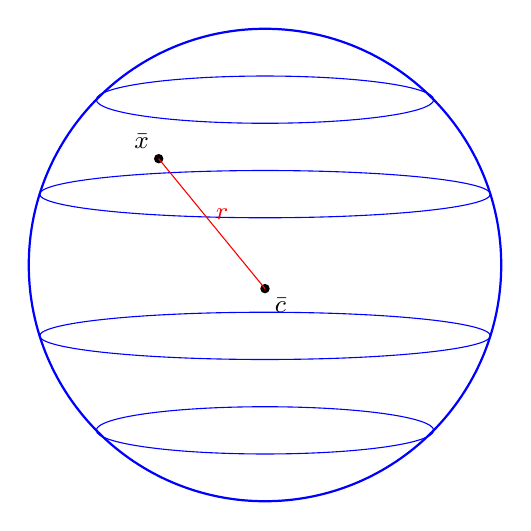
\begin{tikzpicture}[scale=3]
    

  % Outer Sphere
  \shade[ball color=white, opacity=0.0] (0,0) circle(1); % invisible shading
  \draw[blue, thick] (0,0) circle(1); % sphere boundary

  % Latitude lines (ellipses)
  \foreach \y in {-0.7,-0.3,0.3,0.7}
    \draw[blue, thin] (0,\y) ellipse ({sqrt(1 - \y*\y)} and 0.1);

  % Points
  \coordinate (C) at (0,-0.1);
  \coordinate (X) at (-0.45,0.45);
  \fill (C) circle (0.02) node[below right] {\small$\bar{c}$};
  \fill (X) circle (0.02) node[above left] {\small$\bar{x}$};

  % Radius
  \draw[red, thin] (C) -- (X) node[midway, above right=-2pt] {\small$r$};


\end{tikzpicture}

\end{center}
Our everyday experience tells us that a line intersects a sphere in either one or two points, or not at all. Indeed, if you shoot an arrow at a soccer ball at a very high speed and do not miss, then the arrow will enter the ball at one point and exit at another, or just graze the surface of the ball. We illustrate this fact by means of some examples.

%SphereExamples.tex
%This file is part of the WTW124 course material.

\begin{examplebox}
Let $S$ be the sphere with radius $2$ and centre $\bar{0}$, and $L$ the line through the points $\bar{p} = \langle 3, 1, 0 \rangle$ and $\bar{q} = \langle 0, 0, 3 \rangle$. Determine the points where $L$ intersects $S$, if any such points exist.
\vspace{1em}

\textbf{Solution}
\vspace{1em}

$L$ intersects $S$ at a point $\bar{r}$ if and only if $\bar{r} \in S$ and $\bar{r} \in L$. Therefore $L$ intersects $S$ at $\bar{r}$ if and only if
\[
\bar{r} = t\bar{p} + (1 - t)\bar{q} = \langle 3t, t, 3 - 3t \rangle \quad \text{for some } t \in \mathbb{R}
\]
and
\[
\|\bar{r} - \bar{0}\| = 2.
\]
It is convenient to replace the last equation with
\[
\|\bar{r} - \bar{0}\|^2 = 4.
\]
Substituting the expression for $\bar{r}$ we get
\[
4 = \|\bar{r} - \bar{0}\|^2 = \| \langle 3t, t, 3 - 3t \rangle \|^2 = 9t^2 + t^2 + 9 - 18t + 9t^2.
\]
Hence
\[
19t^2 - 18t + 5 = 0.
\]
Because the discriminant of the quadratic equation satisfies
\[
\Delta = (-18)^2 - 4 \cdot 19 \cdot 5 = -56 < 0,
\]
equation has no real solutions. Therefore the line $L$ does not intersect the sphere $S$.
\end{examplebox}

\begin{examplebox}
Let $S$ be the sphere with radius $1$ and centre $\bar{c} = \langle 1, 1, 1 \rangle$, and $L$ the line through the points $\bar{p} = \langle 2, -1, 1 \rangle$ and $\bar{q} = \langle -1, 2, 1 \rangle$. Determine the points where $L$ intersects $S$, if any such points exist.
\vspace{1em}

\textbf{Solution}
\vspace{1em}

A point $\bar{r}$ lies on both $L$ and $S$ if and only if $\bar{r} \in S$ and $\bar{r} \in L$. Therefore $L$ intersects $S$ at $\bar{r}$ if and only if
\[
\bar{r} = t\bar{p} + (1 - t)\bar{q} = \langle 3t - 1, 2 - 3t, 1 \rangle \quad \text{for some } t \in \mathbb{R}
\]
and
\[
\|\bar{r} - \bar{c}\| = 1.
\]
In order to simplify our calculations, we replace this equation with
\[
\|\bar{r} - \bar{c}\|^2 = 1.
\]
Substituting, we find
\[
1 = \| \bar{r} - \bar{c} \|^2 = \| \langle 3t - 2, 1 - 3t, 0 \rangle \|^2 = 9t^2 - 12t + 4 + 1 - 6t + 9t^2.
\]
Hence
\[
18t^2 - 18t + 4 = 0.
\]
Solving, we find $t = \frac{2}{3}$ or $t = \frac{1}{3}$. Substituting these into the expression for $\bar{r}$:
\[
\bar{r}_0 = \langle 3 \cdot \tfrac{2}{3} - 1, 2 - 3 \cdot \tfrac{2}{3}, 1 \rangle = \langle 1, 0, 1 \rangle,
\]
\[
\bar{r}_1 = \langle 3 \cdot \tfrac{1}{3} - 1, 2 - 3 \cdot \tfrac{1}{3}, 1 \rangle = \langle 0, 1, 1 \rangle.
\]
\end{examplebox}

\begin{examplebox}
Let $S$ be the sphere with radius $\sqrt{2}$ and centre $\bar{c} = \langle 1, 0, 1 \rangle$, and $L$ the line through the points $\bar{p} = \langle -2, 2, 2 \rangle$ and $\bar{q} = \langle 1, -1, -1 \rangle$. Determine the points where $L$ intersects $S$, if any such points exist.
\vspace{1em}

\textbf{Solution}
\vspace{1em}

$L$ intersects $S$ at a point $\bar{r}$ if and only if $\bar{r} \in S$ and $\bar{r} \in L$. Therefore $L$ intersects $S$ at $\bar{r}$ if and only if
\[
\bar{r} = t\bar{p} + (1 - t)\bar{q} = \langle 1 - 3t, 3t - 1, 3t - 1 \rangle \quad \text{for some } t \in \mathbb{R}
\]
and
\[
\|\bar{r} - \bar{c}\| = \sqrt{2}.
\]
It is convenient to replace this with
\[
\|\bar{r} - \bar{c}\|^2 = 2.
\]
Substituting gives
\[
2 = \| \bar{r} - \bar{c} \|^2 = \| \langle -3t, 3t - 1, 3t - 2 \rangle \|^2 = 9t^2 + 9t^2 - 6t + 1 + 9t^2 - 12t + 4.
\]
Hence
\[
27t^2 - 18t + 5 = 2 \Rightarrow 9t^2 - 6t + 1 = 0.
\]
This equation has only one solution, namely $t = \frac{1}{3}$. Therefore the line $L$ intersects the sphere $S$ at precisely one point:
\[
\bar{r} = \langle 1 - 3 \cdot \tfrac{1}{3}, 3 \cdot \tfrac{1}{3} - 1, 3 \cdot \tfrac{1}{3} - 1 \rangle = \langle 0, 0, 0 \rangle = \bar{0}.
\]
\end{examplebox}


\begin{exercisebox}
1. Let $L$ be the line through $\bar{p}$ and $\bar{q}$. In each case, determine whether or not the given points $\bar{a}$ and $\bar{b}$ are on $L$. If one or both of the points is on $L$, also determine whether or not the point is between $\bar{p}$ and $\bar{q}$.
\begin{itemize}
    \item[(a)] $\bar{p} = \langle 2, 2, -3 \rangle$, $\bar{q} = \bar{0}$; $\bar{a} = \langle 1, 1, -2 \rangle$, $\bar{b} = \langle -4, -4, 6 \rangle$
    \item[(b)] $\bar{p} = \langle 1, 2, 1 \rangle$, $\bar{q} = \langle 1, 0, 2 \rangle$; $\bar{a} = \langle 1, 8, -2 \rangle$, $\bar{b} = \langle 1, 4, 1 \rangle$
    \item[(c)] $\bar{p} = \langle -1, 1, 1 \rangle$, $\bar{q} = \langle 1, 2, 2 \rangle$; $\bar{a} = \langle -5, -1, -1 \rangle$, $\bar{b} = \langle -3, 3, 3 \rangle$
    \item[(d)] $\bar{p} = \langle 2, 3, -5 \rangle$, $\bar{q} = \langle -1, 2, 1 \rangle$; $\bar{a} = \langle 5, 4, -10 \rangle$, $\bar{b} = \langle -4, 3, 7 \rangle$
    \item[(e)] $\bar{p} = \langle 0, 2, -1 \rangle$, $\bar{q} = \langle 1, 0, -1 \rangle$; $\bar{a} = \langle -4, 10, -1 \rangle$, $\bar{b} = \langle -2, 7, -1 \rangle$
\end{itemize}

2. Consider the points $\bar{p} = \langle 1, 0, 1 \rangle$ and $\bar{q} = \langle 4, 2, 6 \rangle$. Determine whether or not the points $\bar{a}, \bar{b}$ and $\bar{c}$ are between $\bar{p}$ and $\bar{q}$, where
\[
\bar{a} = \left\langle \tfrac{5}{2}, 1, \tfrac{7}{2} \right\rangle,\quad \bar{b} = \left\langle 3, \tfrac{4}{3}, \tfrac{13}{3} \right\rangle,\quad \bar{c} = \langle -2, -2, -4 \rangle.
\]

3. Determine whether or not the lines $L_1$ and $L_2$ intersect, and find the point(s) of intersection, if any exist.
\begin{itemize}
    \item[(a)] $L_1$: through $\bar{p} = \langle 1, 2, -1 \rangle$, $\bar{q} = \langle 2, 0, 1 \rangle$; 
              $L_2$: through $\bar{a} = \langle 0, 4, 1 \rangle$, $\bar{b} = \langle -2, 8, -11 \rangle$
    \item[(b)] $L_1$: through $\bar{p} = \langle -1, 0, -1 \rangle$, $\bar{q} = \langle 1, 1, 1 \rangle$; 
              $L_2$: through $\bar{a} = \langle -1, 0, -5 \rangle$, $\bar{b} = \langle 1, 1, -1 \rangle$
    \item[(c)] $L_1$: through $\bar{p} = \langle 1, 2, 1 \rangle$, $\bar{q} = \langle -1, 0, 2 \rangle$; 
              $L_2$: through $\bar{a} = \langle -2, -2, 5 \rangle$, $\bar{b} = \langle -1, -1, 6 \rangle$
    \item[(d)] $L_1$: through $\bar{p} = \langle 2, 0, -1 \rangle$, $\bar{q} = \langle 1, -2, 1 \rangle$; 
              $L_2$: through $\bar{a} = \langle 0, -4, 1 \rangle$, $\bar{b} = \langle 3, 2, -3 \rangle$
    \item[(e)] $L_1$: through $\bar{p} = \langle 2, 1, -2 \rangle$, $\bar{q} = \langle -2, -1, 2 \rangle$; 
              $L_2$: through $\bar{a} = \langle 5, 3, -6 \rangle$, $\bar{b} = \langle 1, 5, -4 \rangle$
    \item[(f)] $L_1$: through $\bar{p} = \langle 2, 3, -1 \rangle$, $\bar{q} = \langle -1, 4, 1 \rangle$; 
              $L_2$: through $\bar{a} = \langle 5, 2, -3 \rangle$, $\bar{b} = \langle -1, 4, 0 \rangle$
\end{itemize}

4. Let $\bar{c} = \langle 1, 0, 0 \rangle$ and let $S$ be the sphere with centre $\bar{c}$ and radius $2$. Determine if the line $L$ intersects the sphere $S$, and find the point(s) of intersection, if any exist.
\begin{itemize}
    \item[(a)] $L$: through $\bar{p} = \langle 1, -2, 2 \rangle$, $\bar{q} = \langle 2, -1, 1 \rangle$
    \item[(b)] $L = \{\langle 3t, 4 - 4t, 1 \rangle : t \in \mathbb{R} \}$
    \item[(c)] $L$: through $\bar{p} = \langle 0, -1, 3\sqrt{2} \rangle$, $\bar{q} = \langle 3, 2, 0 \rangle$
    \item[(d)] $L$: through $\bar{p} = \langle 3, 2\sqrt{3}, -2 \rangle$, $\bar{q} = \langle 0, -\sqrt{3}, 4 \rangle$
\end{itemize}

\end{exercisebox}

\begin{exercisebox}
    
5. Let $L$ be the line through $\bar{p} = \langle 1, 1, -1 \rangle$ and $\bar{q} = \langle -1, 2, 1 \rangle$. For the given points $\bar{a}$ and $\bar{b}$, determine the value(s) of the real number $\alpha$ so that the line through $\bar{a}$ and $\bar{b}$ intersects $L$ at exactly one point.
\begin{itemize}
    \item[(a)] $\bar{a} = \langle 1, 0, 1 \rangle$, $\bar{b} = \langle -3, 1, 3\alpha + 1 \rangle$
    \item[(b)] $\bar{a} = \langle -9, 6, \alpha^2 \rangle$, $\bar{b} = \langle 3, 0, -3 \rangle$
    \item[(c)] $\bar{a} = \langle 1, 0, 1 \rangle$, $\bar{b} = \langle -3, 1, 3\alpha + 1 \rangle$
    \item[(d)] $\bar{a} = \langle 2 + \alpha, 2, 3 \rangle$, $\bar{b} = \langle 2, 1, -1 \rangle$
\end{itemize}

6. For vectors $\bar{a}$ and $\bar{b}$ as given below, sketch the line segments between $\bar{0}$ and $\bar{a}$, $\bar{0}$ and $\bar{b}$, $\bar{a}$ and $\bar{a} + \bar{b}$, and $\bar{b}$ and $\bar{a} + \bar{b}$ in the $xy$-plane $\{ \langle x, y, 0 \rangle : x, y \in \mathbb{R} \}$. Identify the figure formed by the four line segments.
\begin{multicols}{2}
\begin{itemize}
    \item[(a)] $\bar{a} = \langle 1, 0, 0 \rangle$, $\bar{b} = \langle 0, 1, 0 \rangle$
    \item[(b)] $\bar{a} = \langle 1, 2, 0 \rangle$, $\bar{b} = \langle 2, 1, 0 \rangle$
    \item[(c)] $\bar{a} = \langle -1, 1, 0 \rangle$, $\bar{b} = \langle 2, 1, 0 \rangle$
    \item[(d)] $\bar{a} = \langle 3, 1, 0 \rangle$, $\bar{b} = \langle -2, 3, 0 \rangle$
    \item[(e)] $\bar{a} = \langle 4, 2, 0 \rangle$, $\bar{b} = \langle 2, 1, 0 \rangle$
    \item[(f)] $\bar{a} = \langle 5, 3, 0 \rangle$, $\bar{b} = \langle 2, -3, 0 \rangle$
\end{itemize}
\end{multicols}

7. Determine whether or not the given lines $L_1$ and $L_2$ are parallel.
\begin{itemize}
    \item[(a)] $L_1$: $\bar{x} = \langle 2 + 3t, -t, 2 + t \rangle$, $L_2$: $\bar{x} = \langle 1, 3, 1 \rangle + s\langle 6, -2, 2 \rangle$
    \item[(b)] $L_1$: through $\bar{p} = \langle -2, 1, 2 \rangle$, $\bar{q} = \langle 5, 4, -1 \rangle$; 
              $L_2$: $\bar{x} = \langle 8 - 14s, -6s, 1 + 5s \rangle$
\end{itemize}

8. Determine the value(s) of the real number $c$ for which the given lines $L_1$ and $L_2$ are parallel.
\begin{itemize}
    \item[(a)] $L_1$: $\bar{x} = \langle 4 + c^2t, -1, t + 1 \rangle$, $L_2$: $\bar{x} = \langle 4, 2, 1 \rangle + s\langle 4, 0, 2 \rangle$
    \item[(b)] $L_1$: through $\bar{p} = \langle 1, 2c, 0 \rangle$, $\bar{q} = \langle -1, 1, 1 \rangle$; 
              $L_2$: through $\bar{a} = \langle 0, 1, 1 \rangle$, $\bar{b} = \langle 1, 2, -1 \rangle$
    \item[(c)] $L_1$: through $\bar{p} = \langle c^2, 1, 1 \rangle$, $\bar{q} = \langle -1, 0, 2 \rangle$; 
              $L_2$: through $\bar{a} = \langle 3, 4, c \rangle$, $\bar{b} = \langle -1, 2, 3 \rangle$
    \item[(d)] $L_1$: $\bar{x} = \langle 1 + ct, 2, 2t + 1 \rangle$, $L_2$: $\bar{x} = \langle 2, 5, -3 \rangle + s\langle 1, 3, -1 \rangle$
    \item[(e)] $L_1$: $\bar{x} = \langle c + t, 2t - c, c - 3t \rangle$, $L_2$: $\bar{x} = \langle -2, 0, 3 \rangle + s\langle -2, -4, 6 \rangle$
\end{itemize}
\end{exercisebox}

Now that we have properly defined lines in space, we can now move onto to more specific concepts in space; in particular we will look at angles and measurements
\newpage

